\chapter{WLAN technologies and security}
With WLAN, as previously mentione, we refer to a network that covers a small area. Actually, the most
common WLAN technolgy is Wi-Fi, which is based on IEEE 802.11 and trademarked.\\
Wifi supports mainly the infrastrcuture-based mode: which is usually made up of 
\begin{itemize}
  \item Access Points(APs)
  \item Wireless stations(STAs)
\end{itemize}
All the STAs are connected to the APs, which are connected to the wired network.\\
It actually supports ad-hoc mode, which uses direct communication, but it is not used that much.\\
  In infrastructure-based mode, all traffic must go through the AP, having no direct communication 
  possible. This is to solve the hidden terminal problem, where two STAs can't communicate because they
  can't hear each other, and 
\begin{figure}[h]
  \centering
  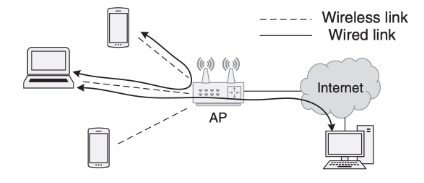
\includegraphics[width=0.7\textwidth]{img/wireless/wlan communication.png}
  \caption{Schema of a possible wireless communication}
\end{figure}
Furthermore, because it is based on 802.11, it carries over most of the standard:
\begin{itemize}
  \item \textbf{half-duplex communication channel}, so at any time only one station can transmit or receive
  \item works on 2.4GHz and 5GHz bands, so multiplexing is available but quite limited
  \item uses \textbf{CSMA/CA} for medium access(carrier sense multiple access with collision avoidance)
\end{itemize}
The spectrum of the 2.4GHz band is divided into 14 channels, but only 3 of them are non-overlapping.
The 5GHz band has more channels, but it is less used because of the shorter range.
\begin{figure}
  \centering
  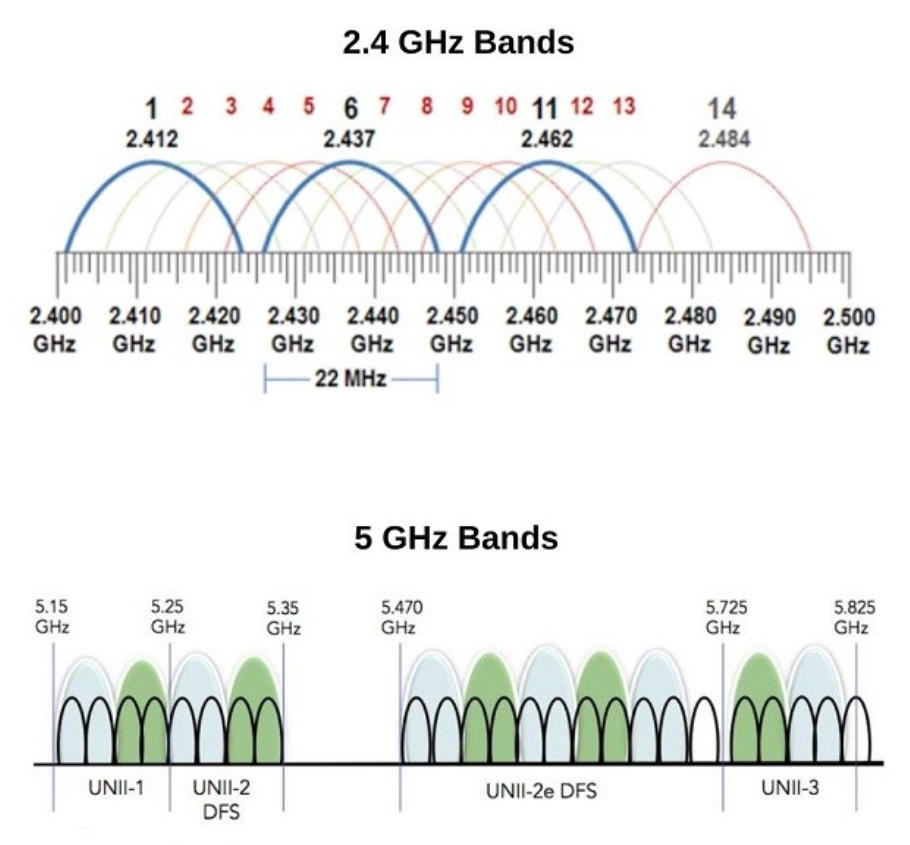
\includegraphics[width=0.5\textwidth]{img/wireless/80211 channels.png}
  \caption{802.11 channels}
\end{figure}
\begin{section}{WLAN Access}
  Before being able to access the network, the STA must go through the following steps:
  \begin{enumerate}
    \item \textbf{Scanning}: the STA scans the environment to find the APs
    \item \textbf{Association}: the STA selects the AP and sends an association request
    \item \textbf{Authentication}: the AP sends an authentication request to the STA
    \item \textbf{Authentication}: the STA sends an authentication response to the AP
    \item \textbf{Association}: the AP sends an association response to the STA
    \item \textbf{Exchange of data}: the STA can now exchange data with the AP
  \end{enumerate}
  For what concerns the scanning and association, the access point sends a beacon frame every 100 ms, which contains
  the SSID, the supported data rates, the supported security protocols, and the channel number.\\
  The STA can then send a probe request to the AP, which will respond with a probe response.\\
\end{section}


